%%%%%%%%%%%%%%%%%%%%%%% file typeinst.tex %%%%%%%%%%%%%%%%%%%%%%%%%
%
% This is the LaTeX source for the instructions to authors using
% the LaTeX document class 'llncs.cls' for contributions to
% the Lecture Notes in Computer Sciences series.
% http://www.springer.com/lncs       Springer Heidelberg 2006/05/04
%
% It may be used as a template for your own input - copy it
% to a new file with a new name and use it as the basis
% for your article.
%
% NB: the document class 'llncs' has its own and detailed documentation, see
% ftp://ftp.springer.de/data/pubftp/pub/tex/latex/llncs/latex2e/llncsdoc.pdf
%
%%%%%%%%%%%%%%%%%%%%%%%%%%%%%%%%%%%%%%%%%%%%%%%%%%%%%%%%%%%%%%%%%%%


\documentclass[runningheads,a4paper]{llncs}

\usepackage{amssymb}
\setcounter{tocdepth}{3}
\usepackage{graphicx}
\usepackage{hyperref}
\usepackage{amsmath}
\usepackage{listings}

\usepackage{tikz}
\usetikzlibrary{positioning,arrows,shapes.geometric,
	matrix,shapes.symbols,decorations.pathreplacing}

\usepackage{subcaption}
\captionsetup{compatibility=false}

\usepackage{booktabs}

\usepackage[utf8]{inputenc}
\usepackage[T1]{fontenc}
\usepackage{lmodern}

\usepackage{url}
\urldef{\mailsa}\path|loic_tetrel@yahoo.fr|
\newcommand{\keywords}[1]{\par\addvspace\baselineskip
	\noindent\keywordname\enspace\ignorespaces#1}

\begin{document}
	
	\mainmatter  % start of an individual contribution
	
	% first the title is needed
	\title{Gaussian Process}
	
	% a short form should be given in case it is too long for the running head
	\titlerunning{Gaussian Process}%
	
	% the name(s) of the author(s) follow(s) next
	%
	% NB: Chinese authors should write their first names(s) in front of
	% their surnames. This ensures that the names appear correctly in
	% the running heads and the author index.
	%
	\author{Loïc Tetrel}
	%
	\authorrunning{Gaussian Process}
	% (feature abused for this document to repeat the title also on left hand pages)
	
	% the affiliations are given next; don't give your e-mail address
	% unless you accept that it will be published
	%\institute{******************************************\\
	\institute{}
	
	%
	% NB: a more complex sample for affiliations and the mapping to the
	% corresponding authors can be found in the file "llncs.dem"
	% (search for the string "\mainmatter" where a contribution starts).
	% "llncs.dem" accompanies the document class "llncs.cls".
	%
	
	\toctitle{Gaussian Process}
	
	\maketitle

	\keywords{Generative model; Filtering; Regression}

	\section{Introduction}\label{introduction}
	Daniel G. Kringe was the first to define a Gaussian Process in a new interpolation method to evaluate mining ressources in geostatistics. In this time, we were talking about Kriging \cite{krige1951statistical}. Later, Rasmussen\cite{rasmussen2006gaussian} propose to develop the Gaussian Process ($\mathcal{GP}$) theory to do machine learning. Since then, it is a famous generative model for AI applications.
	\section{Theory}\label{theory}
	The function $f$ is a $\mathcal{GP}$ if a subset of the outputs $\{y(x_0),...,y(x_N)\}$ has a multivariate gaussian distribution :
	
	\begin{equation}
	f(x_0,..., x_N) = \mathcal{N}(\mu, \Sigma),
	\end{equation}
		
	This process is entirely define by its mean function $\mu$ ans its covariance $\Sigma$.
	
	\begin{equation}
	\mathbf{\mu} = 
	\begin{bmatrix}
	\mu_0\\
	\vdots\\
	\mu_N\\
	\end{bmatrix};
	\qquad 
	\Sigma = 
	\begin{bmatrix}
	\Sigma(x_0,x_0) & \dots & \Sigma(x_0,x_N) \\
	\vdots & \ddots & \vdots \\
	\Sigma(x_N,x_0) & \dots & \Sigma(x_N,x_N) \\
	\end{bmatrix}.
	\end{equation}
	
	Usually, a gaussian noise is employed to model the uncertainty behind the model, so the output becomes : 
	
	\begin{equation}
	y = f(x) + \mathcal{N}(0, \sigma_{y} ^2).
	\end{equation}
	
	The covariance allows us to model the non-linearity of the inputs (known as the kernel trick). A widely used kernel is the gaussian one, which will ensure that close inputs produce output values that are close together :
	
	\begin{equation}
	\Sigma(x,x') =\sigma_x \exp \bigg(\frac{\| x - x'\|^2}{2l^2}\bigg).
	\end{equation}
	
	Where $\sigma_x$ is the noise from the inputs, and $l$ is the lengthscale of the covariance. This length has to be
	choose carefully to improve accuracy of the prediction.
	\par An important thing to understand is to distinguish the prior and the posterior of the $\mathcal{GP}$. The prior is observable whenever we have training values, the posterior will change in consequence with new data coming into the process.
	
	\section{Code example}\label{example}
	Below you can see the effect on the $\mathcal{GP}$ when some inputs comes.
	You may notice that the outputs from the prior (vertical axis) are coming from a gaussian distribution :
	
	\begin{figure}
		\centering
		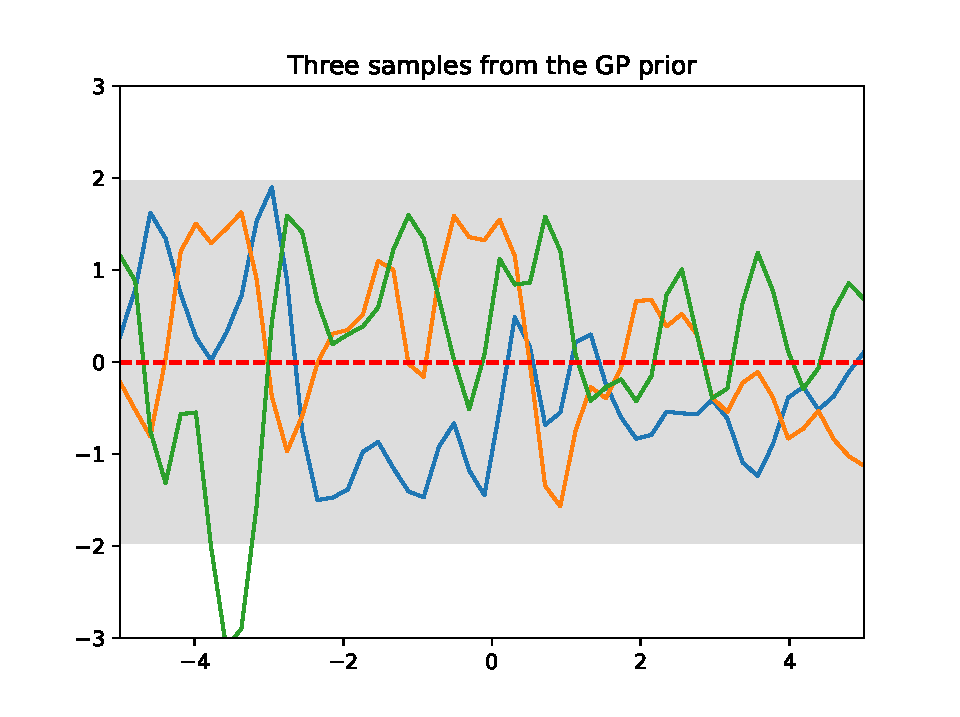
\includegraphics[width=0.5\textwidth]{Figures/GPprior}
		\\ \parbox{0.75\textwidth}{\caption[Gaussian Process prior]{Three random function taken from the prior. The mean function (red) is zero, and the covariance function constant.}\label{fig:GPprior}} 
	\end{figure}
	
	\begin{figure}
		\centering
		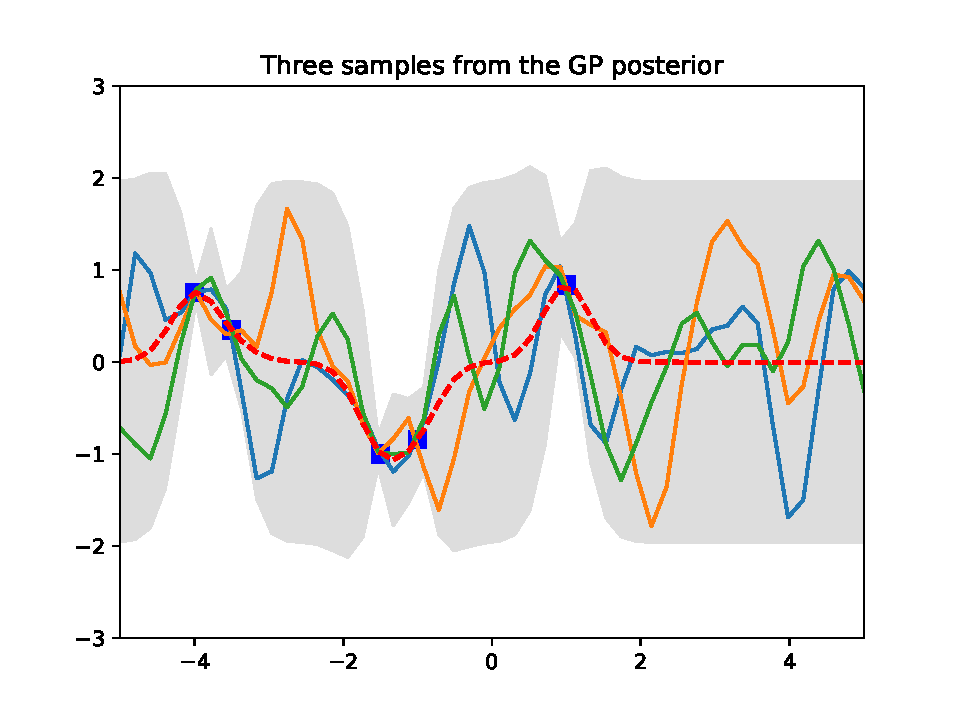
\includegraphics[width=0.5\textwidth]{Figures/GPposterior}
		\\ \parbox{0.75\textwidth}{\caption[Gaussian Process posterior]{With 5 test data (blue squares), three different samples are taken from the posterior. We can now evaluate the mean function (red) and the covariance at 95\% (grey). }\label{fig:GPposterior}} 
	\end{figure}
	
	To generate the figure, you can use this code (slightly modified from \url{http://katbailey.github.io/post/gaussian-processes-for-dummies/}):
	
	\lstinputlisting[language=python]{PriorPosterior.py}
	
	\section{Study case}
	\label{sec:method}
	
	\section{Conclusion}
	\label{sec:conclusion}
	
	 
	\subsection*{Acknowledgment}
	Thanks
	
	{\small
		\bibliographystyle{splncs03}
		\bibliography{article}
	}
	
\end{document}

